\chapter{Bausteinsicht}
In diesem Abschnitt wird die Architektur der Middleware beschrieben.

\section{Allgemein}
Grundlage der Architektur ist eine 3-Layer-Architektur. In dieser ist die Applikation die oberste Schicht, die Middleware die Mittlere Schicht und die OS/Runtime die unterste Schicht. Die Middleware besteht aus einem 2-Tier-Schichten-Modell. Diese ist ein Client-Server-Architektur \textcolor{red}{TODO:Quelle}. Diese Architektur ist eine zustandslose Design, das Skalierbarkeit, Wartbarkeit und Fehlertoleranz dadurch  fördert, dass die einzelnen Nachrichten keinen Bezug zueinander haben\textcolor{red}{TODO:Quelle}.

\section{Beschreibung Client- / Server-Stubs}
Jeder Teilnehmer, der die Middleware nutzt hat einen Client-Stub und einen Server-Stub. Als Schnittstelle zur Applikation dient jeweils ein Applikationsstub. Der Applikations-Stub auf Client Seite implemetiert die aufrufenden Funktionen der entfernten Applikation, indem es im Rumpf der entfernten Funktion die Schnittstellen-Funktion "invoke" aufruft. Diese Funktion ist im Client-Stub implementiert. In der Funktion wird der RPC-Call zunächst durch Marshalling serialisert und mit einem UDP Paket verschickt.\\\\
Der Server-Stub empfängt die RPC-Aufrufe über UDP. Das Paket wird im Server-Stub unmarshalled und dann wird die "call"-Funktion aufgerufen. Die "call"-Funktion wird im Applikation-Stub auf der Server Seite implementiert. Dort wird per Callback-Pattern die Funktion der lokalen Applikation aufgerufen. Das wird bei asynchronen RPC-Aufrufen bevorzugt \textcolor{red}{TODO:Quelle}.

\section{Namensauflösung}
Es gibt einen zentralen Namensauflösungsdienst \textcolor{red}{TODO:Quelle}. Dieser implementiert die Funktion "register" und "resolve". \textcolor{red}{TODO:Abschnitt}\textcolor{red}{TODO:Korrektur Funcktionsnamen}. Der Client des Aufrufers implementiert einen Caching-Proyx \textcolor{red}{TODO:Quelle}, um die Netzwerklast zu reduzieren und um die Verteilungstransparenz zu fördern\textcolor{red}{TODO:Quelle}, da nur der Caching-Proxy den Namensserver kennt. Der Caching-Proxy implementiert die Funktion "resolved"\textcolor{red}{TODO:Korrektur Funktionsnamen}. Der Aufruf von "resolve\" ist synchron. Jeder Eintrag ist für 5 Minuten valide. Damit wird aktzeptiert, dass die Daten für die Auflösung inkonsistent sein kann. Dient aber der Echtzeitanforderung und der Safetyanforderung an die Applikation.

\section{Watchdog}


\newcommand{\comment}[1]{}

\comment{
	@startuml
	title Middleware-Komponenten – Asynchrones RPC (ohne Anwendung)
	
	package "Client-Middleware" {
		[Client-Proxy]
		[Marshalling]
		[Async RPC Sender]
		
		
	}
	
	package "Middleware Infrastruktur" {
		[Naming Service]
		[Message Transport]
	}
	
	[Client-Proxy] --> [Naming Service] : Dienstadresse auflösen
	[Client-Proxy] --> [Marshalling] : Argumente serialisieren
	[Marshalling] --> [Async RPC Sender] : Anfrage senden
	package "Server-Middleware" {
		[Async RPC Receiver]
		[Unmarshalling]
		[Server-Skeleton]
		
		[Async RPC Receiver] --> [Unmarshalling] : Deserialisieren
		[Unmarshalling] --> [Server-Skeleton] : Methodenaufruf
	}
	
	
	[Async RPC Sender] --> [Message Transport]
	[Message Transport] --> [Async RPC Receiver]
	@enduml
}

\begin{figure}[htbp]
	\centering
	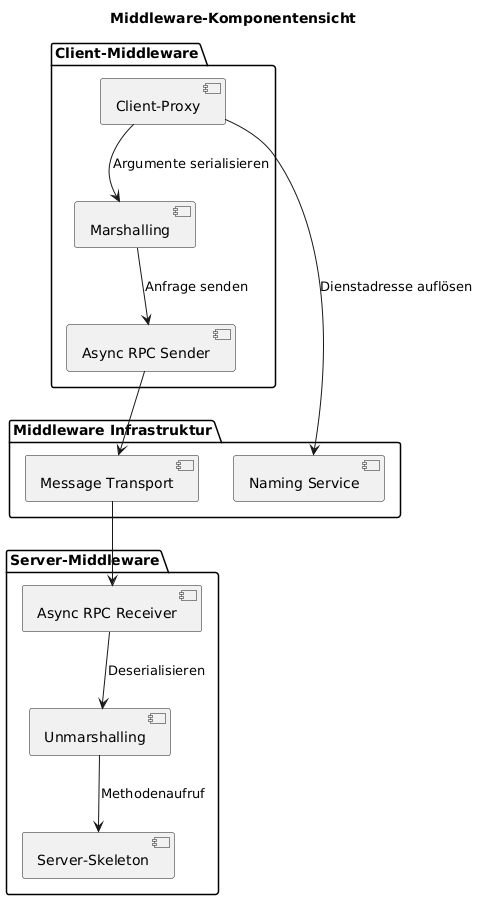
\includegraphics[width=0.8\textwidth]{diagrams/bausteinsicht.png}
	\caption{Komponenten der Middleware}
	\label{fig:meine-abbildung}
\end{figure}


\section*{Beschreibung}